\documentclass[11pt]{article}
\usepackage[english]{babel}
\usepackage[T1]{fontenc}
\usepackage[utf8]{inputenc}
\usepackage{amsmath,amssymb,amsthm,geometry}
\usepackage{graphicx}
\usepackage{tikz}
\usetikzlibrary{calc}
\usepackage{hyperref}
\geometry{margin=2.5cm}

\title{The Dodecagram Polygonal Theorem}
\author{Jose Eugenio A. G.}
\date{02/19/2026}

\newtheorem{theorem}{Theorem}
\newtheorem{lemma}{Lemma}
\newtheorem{definition}{Definition}
\newtheorem{corollary}{Corollary}

\begin{document}
\maketitle

\begin{abstract}
We characterize a critical family of regular star polygons described by the Schläfli symbol $\{n/k\}$. Under the Diophantine relation $k = n/2 - 1$, we establish The Dodecagram Polygonal Theorem, proving that the regular dodecagram $\{12/5\}$ is the last polygon for which all non-convex internal stellation rings are composite in the sense of $\gcd(n,s)>1$. This establishes $\{12/5\}$ as a sharp arithmetic and combinatorial threshold in the theory of regular stellations.
\end{abstract}

\section{Introduction}

Regular star polygons constitute a classical topic in Euclidean geometry and are denoted by the Schläfli symbol $\{n/k\}$. Their stellations generate internal rings whose components may be simple polygons, star polygons, or unions of multiple regular polygons.

In this paper we introduce a critical arithmetic relation between $n$ and $k$ and show that the dodecagram $\{12/5\}$ occupies a unique structural position: it is the last polygon in this family whose non-convex internal rings are all composite. This property follows from elementary number-theoretic constraints rather than geometric coincidence.

\section{Preliminaries}

\begin{definition}
A \emph{regular star polygon} $\{n/k\}$ consists of $n$ equally spaced vertices on a circle, with edges joining each vertex to the $k$-th subsequent vertex, where $\gcd(n,k)=1$ and $1<k<n/2$.
\end{definition}

\begin{definition}
An \emph{internal ring} of $\{n/k\}$ is the orbit, under the action of the dihedral group $D_n$, of intersection points of pairs of non-adjacent edges that lie on a common concentric circle. Rings are indexed from the exterior to the interior.
\end{definition}

\begin{definition}
A ring with step size $s$ is \emph{composite} if $\gcd(n,s)>1$, in which case it consists of $\gcd(n,s)$ congruent regular polygons. A ring is \emph{simple} if $\gcd(n,s)=1$.
\end{definition}

\section{Critical Diophantine Relation}

We impose the Diophantine condition
\begin{equation}
k = \frac{n}{2} - 1, \qquad n = 2(k+1).
\label{eq:critical}
\end{equation}

\section{Main Result}

\begin{theorem}[Dodecagram Polygonal Theorem]
Let $\{n/k\}$ be a regular star polygon satisfying $k = n/2 - 1$. Then:
\begin{enumerate}
\item The polygon has exactly $k-1$ internal rings with step sizes $s=k-1,\dots,2,1$.
\item The two integer solutions $(n,k)$ for which all rings with $s\ge 2$ are composite are $(n,k)=(8,3)$. and $(n,k)=(12,5)$.
\item The only composite ring of $\{8/3\}$ decompose into two squares; the innermost ring is the convex octagon.
\item The three composite rings of $\{12/5\}$ decompose respectively into four equilateral triangles, three squares, and two regular hexagons; the innermost ring is the convex dodecagon.
\end{enumerate}
\end{theorem}

\section{Proofs}

\begin{lemma}
If $k=n/2-1$ and $\gcd(n,k)=1$, then $k$ is odd.
\end{lemma}

\begin{proof}
Since $n=2(k+1)$, we have $\gcd(n,k)=\gcd(2(k+1),k)=\gcd(2,k)$. Hence $\gcd(n,k)=1$ if and only if $k$ is odd.
\end{proof}

\begin{lemma}
A ring of step size $s$ in $\{n/k\}$ is composite if and only if $\gcd(n,s)>1$.
\end{lemma}

\begin{proof}
If $d=\gcd(n,s)>1$, the traversal closes after $n/d$ steps, yielding $d$ congruent regular polygons. If $d=1$, all vertices are visited before closure, yielding a single polygon.
\end{proof}


\begin{lemma}[Ring Structure]
\label{lem:rings}
Let $P_i^{(m)}$ denote the intersection of edge $i$ with edge $i+m$ in $\{n/k\}$,
for $1\le m\le k-1$ and indices taken mod $n$. Then:
\begin{enumerate}
\item[(a)] The $n$ points $\{P_i^{(m)}\}_{i=0}^{n-1}$ lie equally spaced on a circle of radius $r_m$, with $r_1 < r_2 < \cdots < r_{k-1}$.
\item[(b)] The ring $m$ has step $s=m$: the points $P_i^{(m)}$ and $P_{i+m}^{(m)}$ are connected by a segment of edge $i+m$.
\item[(c)] The $j$-th ring from the exterior has step $s = k-j$.
Thus $\{n/k\}$ has exactly $k-1$ internal rings.
\end{enumerate}
\end{lemma}

\begin{proof}
\textbf{(a)} The $n$-fold rotational symmetry $R$ (rotation by $2\pi/n$) satisfies $R(P_i^{(m)}) = P_{i+1}^{(m)}$, so the $n$ points are equally spaced on a circle of radius $r_m = |P_0^{(m)}|$. Parameterizing the edges and solving the resulting $2\times 2$ linear system shows $r_m$ is strictly increasing in $m$.

\textbf{(b)} Both $P_0^{(m)}$ and $P_m^{(m)}$ lie on edge $m$:
$P_0^{(m)}$ is the intersection of edge $0$ \emph{with} edge $m$,
and $P_m^{(m)}$ is the intersection of edge $m$ \emph{with} edge $2m$.
These are the only two intersections of edge $m$ with the ring of radius $r_m$, and the segment of edge $m$ between them is an edge of ring $m$.
Since $P_i^{(m)}$ occupies angular position $i$ (in units of $2\pi/n$),
the step from $P_0^{(m)}$ to $P_m^{(m)}$ is $s = m$.

\textbf{(c)} By (a), the outermost ring is $m=k-1$ and the innermost is $m=1$. The $j$-th ring from the exterior is $m = k-j$, with step $s = k-j$.
\end{proof}

\begin{lemma}[Uniqueness]
Let $k$ be odd and $n=2(k+1)$. Then $\gcd(n,s)>1$ for all $s\in\{2,\dots,k-1\}$ if and only if $(n,k)=(12,5)$ or $(n,k)=(8,3)$.
\end{lemma}

\begin{proof}
The condition requires that every integer in $\{2,\dots,k-1\}$ shares a prime factor with $n=2(k+1)$. Equivalently, letting $p_0$ be the smallest prime not dividing $n$, we need $p_0\ge k$.

\textbf{Case $(n,k)=(8,3)$:} The prime factor of $8=2^3$ is $2$. The unique factor shared with $8$ is $2$, and $p_0=3=k$. \checkmark

\textbf{Case $(n,k)=(12,5)$:} The prime factors of $12=2^2\cdot 3$ are $\{2,3\}$. Each element of $\{2,3,4\}$ shares a factor with $12$, and $p_0=5=k$. \checkmark

\textbf{Case $k\ge 7$:} We show $p_0 < k$ by exhaustive sub-case analysis.
\begin{itemize}
\item If $3\nmid n$: then $p_0=3$. Since $k\ge 7>3$, we have $p_0<k$.
\item If $3\mid n$ but $5\nmid n$: then $p_0=5$. Since $k\ge 7>5$, we have $p_0<k$.
\item If $3\mid n$ and $5\mid n$ but $7\nmid n$: then $p_0=7$. Since $15\mid(k+1)$, we get $k\ge 29>7=p_0$.
\item In general: suppose the primes $3,5,\dots,q$ all divide $n$, and $q'\nmid n$ where $q'$ is the next prime after $q$. Then $2\cdot 3\cdot 5\cdots q\mid(k+1)$, so $k\ge 2\cdot 3\cdot 5\cdots q - 1$. For $q\ge 5$, this bound exceeds $q'$ (since $q'>q$ and $2\cdot 3\cdot 5>5$), giving $p_0=q'<k$.
\end{itemize}
In every sub-case, the smallest prime $p_0$ not dividing $n$ satisfies $p_0<k$, so $s=p_0\in\{2,\dots,k-1\}$ gives $\gcd(n,p_0)=1$, a simple ring. \checkmark
\end{proof}

\section{Geometric Structure and Figures}

\begin{figure}[ht]
\centering
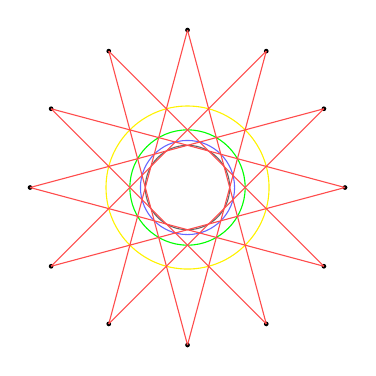
\begin{tikzpicture}[scale=2]
\draw[yellow!100] (0,0) circle (0.517638);
\draw[green!100] (0,0) circle (0.366025);
\draw[blue!60] (0,0) circle (0.298858);
\draw[black!60] (0,0) circle (0.2679);

\foreach \i in {0,...,11} {
\coordinate (P\i) at (90-30*\i:1);
\fill (P\i) circle (0.015);
}

\foreach \i in {0,...,11} {
\pgfmathtruncatemacro{\j}{mod(\i+5,12)}
\draw[red!70] (P\i) -- (P\j);
}
\end{tikzpicture}
\caption{Regular dodecagram $\{12/5\}$ with schematic internal rings.}
\end{figure}

\begin{figure}[ht]
\centering
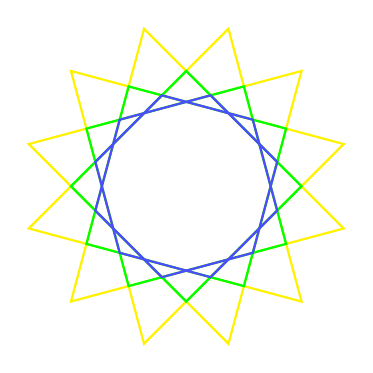
\begin{tikzpicture}[scale=4]
% Four equilateral triangles at r=0.517638 (ring 1, step s=4)
% Vertices of ring 1 are offset 15 degrees from the horizontal
\foreach \i in {15,45,75,105} {
\draw[yellow!100,thick] (\i:0.517638) -- (\i+120:0.517638) -- (\i+240:0.517638) -- cycle;
}
% Three squares at r=0.366025 (ring 2, step s=3)
% Vertices of ring 2 are at 0,30,60,...
\foreach \i in {0,30,60} {
\draw[green!100,thick] (\i:0.366025) -- (\i+90:0.366025) -- (\i+180:0.366025) -- (\i+270:0.366025) -- cycle;
}
% Two regular hexagons at r=0.298858 (ring 3, step s=2)
% Vertices of ring 3 are offset 15 degrees
\foreach \i in {15,45} {
\draw[blue!70!,thick] (\i:0.298858) -- (\i+60:0.298858) -- (\i+120:0.298858) -- (\i+180:0.298858) -- (\i+240:0.298858) -- (\i+300:0.298858) -- cycle;
}
\end{tikzpicture}
\caption{Composite rings of $\{12/5\}$: four equilateral triangles (yellow, $r_3$),
three squares (green, $r_2$), and two regular hexagons (blue, $r_1$).
Vertex positions match the exact intersection radii and angular offsets.}
\end{figure}

\section{Discussion}

The dodecagram appears as a minimal arithmetic configuration in which the prime factors of $n$ cover the full interval of ring step sizes. This property does not persist for larger $n$, where simple stellations inevitably appear. Thus $\{12/5\}$ constitutes a sharp transition point between fully composite and mixed stellation regimes.

\section{Conclusion}

We have proven that $\{12/5\}$ is the last regular star polygon satisfying $k=n/2-1$ whose non-convex internal rings are all composite. The result follows from elementary number theory and symmetry arguments and suggests further connections between stellation theory and arithmetic geometry.

\section*{Acknowledgments}
The author thanks discussions on stellation theory and discrete geometry that motivated this work.

\end{document}